\documentclass[aps,prl,onecolumn,superscriptaddress,nofootinbib]{revtex4-2}
\usepackage{graphicx}
\usepackage{amsmath,amssymb}
\usepackage{bm}
\usepackage[colorlinks=true,linkcolor=blue,citecolor=blue,urlcolor=blue]{hyperref}

% let figures and tables share pages with text instead of collecting on float-only pages
\setcounter{topnumber}{3}
\setcounter{bottomnumber}{2}
\setcounter{totalnumber}{4}
\renewcommand{\topfraction}{0.9}
\renewcommand{\bottomfraction}{0.8}
\renewcommand{\textfraction}{0.07}
\renewcommand{\floatpagefraction}{0.85}

\begin{document}
	
	\title{Statistical Arbitrage in Cryptocurrencies: Momentum, Reversal and Risk-Parity Combination}
	\author{Yunzhe Liu}
	\affiliation{Wall Street Quants course project}
	\date{October 2026}
	
	\begin{abstract}
		We study momentum and reversal strategies on 13 liquid cryptocurrencies using hourly Binance.US data (2020--2025), net of realistic execution costs of 20~bps per unit traded. Momentum signals are strong before costs but unprofitable when rebalanced every four hours; daily rebalancing combined with a cost-penalized portfolio optimization turns them into tradable strategies. Most apparent short-horizon reversal, including pairs trading, disappears on the far more liquid Binance global data and is attributed to price noise on Binance.US; the only robust reversal is buying the market after a liquidation-driven crash (``fire sale''). A risk-parity combination of cross-sectional momentum, time-series momentum, fire-sale reversal and betting-against-beta achieves an in-sample net Sharpe ratio of 1.43 with a market beta of 0.06, and 1.17 out of sample (Binance global, January 2025 -- October 2026).
	\end{abstract}%
	
	\maketitle
	
	% =====================================================================
	
	\section{Data and backtest conventions}
	\label{app:data}
	
	\textit{Data.} Hourly klines are downloaded from Binance.US with \texttt{python-binance} for January 2020 -- December 2025 and resampled to 4-hour bars. Of 24 large coins we keep the 13 with a median volume of at least \$1{,}000 per hour (BTC, ETH, SOL, ADA, BNB, DOGE, VET, LTC, AVAX, ATOM, XLM, LINK, HBAR) and drop XRP and MATIC because of long gaps. Illiquid coins have stale prices, which create spurious reversal. The filter uses full-sample volume (a mild look-ahead).
	
	\textit{Backtest.} Let $r_{i,t}$ be the return of coin $i$ over the 4-hour bar $t$ (6 bars per day), $N_t$ the number of coins with data at bar $t$, and $m_t = N_t^{-1} \sum_i r_{i,t}$ the return of the \emph{equal-weight market}. Let $w_{i,t}$ be the target weight of coin $i$ decided at the close of bar $t$. Unless stated otherwise, weights are demeaned cross-sectional ranks scaled so that $\sum_i |w_{i,t}| = 1$ (dollar neutral). The position is held from bar $t+\ell$ with $\ell \ge 1$, so there is no look-ahead. Turnover, gross return and net return per bar are
	\begin{equation}
		\mathrm{TO}_t = \sum_i \left| w_{i,t} - w_{i,t-1} \right|, \qquad
		r^{\mathrm{gross}}_t = \sum_i w_{i,t-\ell}\, r_{i,t}, \qquad
		r^{\mathrm{net}}_t = r^{\mathrm{gross}}_t - c\, \mathrm{TO}_{t-\ell} ,
		\label{eq:backtest}
	\end{equation}
	with $c = 20$~bps for market orders (7~bps commission and 13~bps slippage) and $c = 7$~bps for limit orders. The \emph{break-even cost} $\overline{r^{\mathrm{gross}}} / \overline{\mathrm{TO}}$ is the largest cost per unit traded at which a strategy still breaks even. Sharpe ratios are annualized with $365 \times 6 = 2190$ bars per year. The \emph{max drawdown} is the largest fall of the cumulative (summed) net return from its previous peak, so it can exceed 100\% for volatile strategies. \emph{Beta} and \emph{alpha} come from a regression of the 4-hour net returns on a factor $f_t$ (the market $m_t$ or BTC): $\beta = \mathrm{cov}(r^{\mathrm{net}}, f)/\mathrm{var}(f)$, the annual alpha is 2190 times the mean residual $e_t = r^{\mathrm{net}}_t - \beta f_t$, and its $t$-statistic is $\bar e / (s_e/\sqrt{n})$, with $s_e$ the standard deviation of the residuals and $n$ the number of bars.
	
	% =====================================================================
	\section{Momentum: horizon, costs and execution}
	\label{app:momentum}
	
	\textit{Horizon.} Cross-sectional (XS) momentum ranks coins on their average return over the last $h$ hours,
	\begin{equation}
		w_{i,t} \propto \operatorname{rank}_i\big(\bar r^{(h)}_{i,t}\big) - \overline{\operatorname{rank}}_t,
		\label{eq:xs}
	\end{equation}
	where $\bar r^{(h)}_{i,t}$ is the average 4-hour return of coin $i$ over the last $h$ hours, $\overline{\operatorname{rank}}_t$ is the mean rank across coins, and the weights are scaled to $\sum_i |w_{i,t}| = 1$. Without a skip ($\ell = 1$ in Eq.~(\ref{eq:backtest}): the position is held from the bar right after the signal), short horizons are strongly negative ($h = 4$: Sharpe $-4.2$): over a few hours coins reverse. Skipping one bar ($\ell = 2$: the bar right after the signal is skipped and the position is held from the next one) removes this effect and every horizon becomes positive [Fig.~\ref{fig:horizon}], so all momentum signals use a one-bar skip, analogous to 12-1 stock momentum.
	
	\begin{figure}[!htbp]
		\centering
		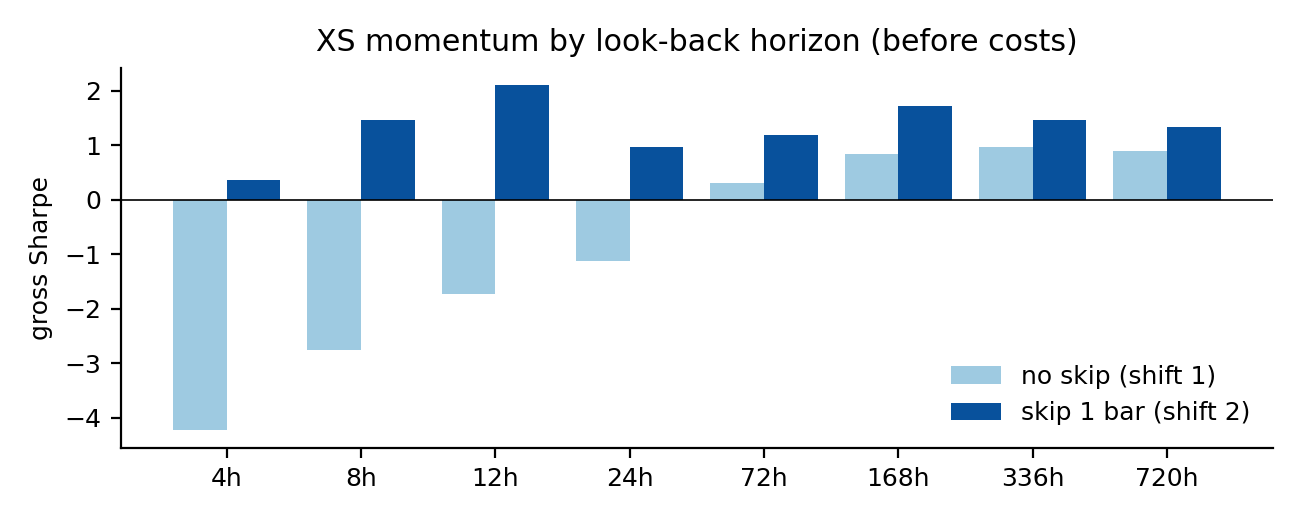
\includegraphics[width=0.75\linewidth]{figures/f1_horizon.png}
		\caption{Gross Sharpe ratio of XS momentum by look-back horizon, with and without skipping the most recent bar.}
		\label{fig:horizon}
	\end{figure}
	
	\textit{Costs.} Rebalanced every 4 hours, every horizon loses money after costs (Table~\ref{tab:costs}). The signal works; the problem is turnover.
	
	\begin{table}[!htbp]
		\caption{XS momentum rebalanced every 4 hours.}
		\label{tab:costs}
		\begin{ruledtabular}
			\begin{tabular}{lcccc}
				Horizon & Gross Sharpe & Net Sharpe (20 bps) & Turnover per bar & Break-even (bps) \\
				\hline
				$h = 24$  & 0.98 & $-7.40$ & 0.606 & 2.3 \\
				$h = 168$ & 1.71 & $-1.77$ & 0.246 & 9.8 \\
				$h = 720$ & 1.34 & $-0.35$ & 0.116 & 15.9 \\
			\end{tabular}
		\end{ruledtabular}
	\end{table}
	
	\textit{Execution.} Rebalancing once a day cuts turnover by about $3\times$ for the slow signal with almost no loss of gross Sharpe ($1.34 \to 1.32$); the result is insensitive to the rebalance hour (0.60--0.80). We then solve, every day at 00:00~UTC,
	\begin{equation}
		\min_{\bm w}\; (\bm w - \bm w^{*})^{\top} \bm\Sigma\, (\bm w - \bm w^{*}) + \lambda\, c\, \lVert \bm w - \bm w' \rVert_1
		\quad \text{s.t.} \quad \textstyle\sum_i w_i = 0,\;\; \lVert \bm w \rVert_1 \le 1,
		\label{eq:opt}
	\end{equation}
	where $\bm w^{*}$ is the momentum (ideal) portfolio, $\bm\Sigma$ is a Ledoit--Wolf covariance estimated on the past 30 days, and $\bm w'$ is the position actually held. The optimizer only trades coins far enough from the ideal portfolio to justify the cost (Table~\ref{tab:opt}); $\lambda = 0$ reproduces the daily rule.
	
	\begin{table}[!htbp]
		\caption{XS momentum ($h = 720$), daily rebalance with the optimization of Eq.~(\ref{eq:opt}).}
		\label{tab:opt}
		\begin{ruledtabular}
			\begin{tabular}{ccccc}
				$\lambda$ & Gross Sharpe & Net Sharpe (20 bps) & Turnover per bar & Break-even (bps) \\
				\hline
				0     & 1.32 & 0.67 & 0.043 & 41 \\
				0.001 & 1.29 & 0.80 & 0.032 & 53 \\
				0.003 & 1.21 & 0.88 & 0.021 & 73 \\
				0.01  & 0.86 & 0.69 & 0.010 & 101 \\
			\end{tabular}
		\end{ruledtabular}
	\end{table}
	
	\textit{Improved signal.} Two changes are made to the ideal portfolio $\bm w^{*}$: the ranks of three horizons (1 week, 2 weeks, 1 month) are averaged instead of picking one, and coins are ranked on volatility-adjusted returns, so that a coin does not rank high just because it is volatile,
	\begin{equation}
		w^{*}_{i,t} \propto \frac{1}{3} \sum_{h \in \{168,\,336,\,720\}} \operatorname{rank}_i\!\left( \frac{\bar r^{(h)}_{i,t}}{\hat\sigma_{i,t}} \right) - \overline{\operatorname{rank}}_t ,
		\label{eq:mhva}
	\end{equation}
	where $\hat\sigma_{i,t}$ is the standard deviation of the 4-hour returns of coin $i$ over the past 30 days, $\overline{\operatorname{rank}}_t$ is the cross-sectional mean of the averaged rank, and the weights are scaled to $\sum_i |w^{*}_{i,t}| = 1$. With the optimization of Eq.~(\ref{eq:opt}) ($\lambda = 0.003$), this raises the gross Sharpe from 1.21 to 1.59 and the net Sharpe from 0.88 to 1.03 [Fig.~\ref{fig:costs}]. This is the final XS strategy.
	
	\begin{figure}[!htbp]
		\centering
		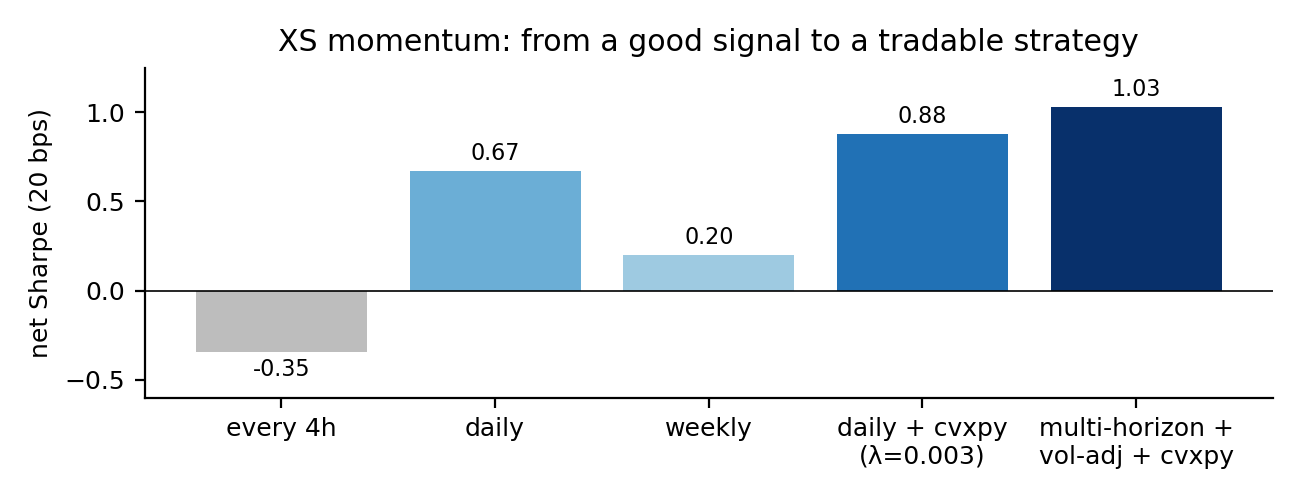
\includegraphics[width=0.75\linewidth]{figures/f2_costs.png}
		\caption{Net Sharpe ratio (20~bps) of XS momentum under successive execution improvements.}
		\label{fig:costs}
	\end{figure}
	
	% =====================================================================
	\section{Momentum and activity (volume)}
	\label{app:volume}
	
	Abnormal volume is defined relative to each coin's own history, $\mathrm{avol}_{i,t} = \overline{V}_{i,t}^{(h)} / \overline{V}_{i,t}^{(90\,\mathrm{d})}$, where $\overline{V}_{i,t}^{(x)}$ is the average 4-hour dollar volume of coin $i$ over the last $x$ (hours or days) up to bar $t$. Let $p_{i,t} = \operatorname{rank}_i(\mathrm{avol}_{i,t}) / N_t \in (0,1]$ be the cross-sectional percentile of abnormal volume, and split the coins into a high-volume half $\mathcal H_t = \{i : p_{i,t} > 1/2\}$ and a low-volume half $\mathcal L_t = \{i : p_{i,t} \le 1/2\}$. Four signals are compared. \emph{Plain} momentum ranks all coins on $\bar r^{(h)}_{i,t}$, as in Eq.~(\ref{eq:xs}). \emph{High avol only} is a long-short momentum portfolio inside $\mathcal H_t$: the coins of $\mathcal H_t$ are ranked among themselves, and the coins of $\mathcal L_t$ get zero weight,
	\begin{equation}
		w_{i,t} \propto
		\begin{cases}
			\operatorname{rank}_{i \in \mathcal H_t}\big(\bar r^{(h)}_{i,t}\big) - \overline{\operatorname{rank}}^{\mathcal H}_t & i \in \mathcal H_t \\
			0 & i \in \mathcal L_t
		\end{cases}
		\label{eq:volhigh}
	\end{equation}
	where $\overline{\operatorname{rank}}^{\mathcal H}_t$ is the mean rank inside $\mathcal H_t$; \emph{low avol only} is the same with $\mathcal H_t$ and $\mathcal L_t$ swapped. \emph{Volume-weighted} momentum keeps all coins but scales the demeaned momentum rank by the volume percentile, so a coin that moved on high volume gets up to twice the weight,
	\begin{equation}
		w_{i,t} \propto \Big( \operatorname{rank}_i\big(\bar r^{(h)}_{i,t}\big) - \overline{\operatorname{rank}}_t \Big) \big( 1 + p_{i,t} \big).
		\label{eq:volw}
	\end{equation}
	All four are scaled to $\sum_i |w_{i,t}| = 1$ and use the same sample (the coins and dates where $\mathrm{avol}_{i,t}$ exists). Consistent with the hypothesis that activity strengthens momentum, momentum among the high-avol half of the coins beats the low-avol half (Table~\ref{tab:volume}; also for $h = 168$: 1.10 vs 0.51). With only 13 coins, however, splitting the universe costs more diversification than the volume information adds, and volume weighting is slightly below plain momentum. Volume is not used in the final strategy.
	
	\begin{table}[!htbp]
		\caption{Volume-conditioned XS momentum, $h = 720$.}
		\label{tab:volume}
		\begin{ruledtabular}
			\begin{tabular}{lcc}
				Signal & Gross Sharpe (every 4h) & Net Sharpe, 20 bps (daily) \\
				\hline
				Plain momentum   & 1.37 & 0.68 \\
				High avol only   & 0.78 & $-0.08$ \\
				Low avol only    & 0.57 & $-0.13$ \\
				Volume-weighted  & 1.32 & 0.64 \\
			\end{tabular}
		\end{ruledtabular}
	\end{table}
	
	% =====================================================================
	\section{Time-series momentum}
	\label{app:ts}
	
	Time-series (TS) momentum goes long all coins (equal weight) if the equal-weight market rose over the last $L$ days and short otherwise. Because single look-backs are noisy, the final signal averages the four signs,
	\begin{equation}
		s_t = \frac14 \sum_{L \in \{7,14,30,60\}} \operatorname{sign}\!\Big(\sum_{j<6L} m_{t-j}\Big), \qquad
		w_{i,t} = \frac{s_t}{N_t},
		\label{eq:ts}
	\end{equation}
	where $6L$ is the number of 4-hour bars in $L$ days. The position $s_t \in [-1, 1]$ is smaller when the look-backs disagree. Unlike XS momentum this strategy is directional, not dollar neutral. It is rebalanced daily with a one-bar skip (Table~\ref{tab:ts}).
	
	\begin{table}[!htbp]
		\caption{Market TS momentum, daily rebalance.}
		\label{tab:ts}
		\begin{ruledtabular}
			\begin{tabular}{lccccc}
				Look-back & Net Sharpe (20 bps) & Annual vol & Max drawdown & Break-even (bps) & Corr.\ with XS \\
				\hline
				7 d   & 0.36 & 80\% & $-1.16$ & 43  & 0.13 \\
				14 d  & 1.11 & 79\% & $-0.85$ & 142 & 0.16 \\
				30 d  & 0.66 & 78\% & $-1.10$ & 115 & 0.15 \\
				60 d  & 0.85 & 76\% & $-1.10$ & 220 & 0.14 \\
				Average 7--60 d & \textbf{0.91} & \textbf{60\%} & $\mathbf{-0.62}$ & 112 & 0.18 \\
			\end{tabular}
		\end{ruledtabular}
	\end{table}
	
	% =====================================================================
	\section{Reversal}
	\label{app:reversal}
	
	Reversal profits are very sensitive to price quality, so each idea is also run on Binance global data for the same coins over 2020--2024. Binance global trades roughly $1000\times$ the volume of Binance.US, and 4-hour returns on the two venues are 96--99\% correlated.
	
	\begin{table}[!htbp]
		\caption{Reversal strategies on Binance.US and Binance global (2020--2024).}
		\label{tab:reversal}
		\begin{ruledtabular}
			\begin{tabular}{llccc}
				Strategy & Data & Gross Sharpe & Net Sharpe (20 bps) & Break-even (bps) \\
				\hline
				4h cross-sectional reversal          & Binance.US     & 3.49 & $-14.84$ & 3.8 \\
				& Binance global & 1.58 & $-17.32$ & 1.7 \\
				Pairs trading (78 pairs, $|z| > 2.5$) & Binance.US     & 1.48 & 0.76     & 41 \\
				& Binance global & 0.72 & $-0.01$  & 20 \\
				Fire sale ($k = 2$, hold 24h)        & Binance.US     & 0.98 & 0.77     & 91 \\
				& Binance global & 1.05 & 0.85     & 108 \\
			\end{tabular}
		\end{ruledtabular}
	\end{table}
	
	\textit{Short-horizon reversal} (the XS momentum weights of Eq.~(\ref{eq:xs}) with $h = 4$ and the sign flipped, no skip, rebalanced every 4 hours) is real but tiny (break-even 2--4~bps), and more than half of its Binance.US profit disappears on clean data.
	
	\textit{Pairs trading.} Following the idea that ``security $A$ minus something correlated to it'' is more mean-reverting, every one of the $\binom{13}{2} = 78$ pairs of coins $(A, B)$ is traded on its log-price spread. With $W = 180$ bars (30 days), the hedge ratio $\beta_t$ is the slope of a rolling regression of $\log P_{A}$ on $\log P_{B}$ over the last $W$ bars, and
	\begin{equation}
		u_t = \log P_{A,t} - \beta_t \log P_{B,t}, \qquad
		z_t = \frac{u_t - \bar u_t}{\sigma_{u,t}}, \qquad
		q_t =
		\begin{cases}
			-1 & z_t > 2.5 \\
			+1 & z_t < -2.5 \\
			\phantom{+}0 & |z_t| < 0.5 \\
			q_{t-1} & \text{otherwise}
		\end{cases}
		\label{eq:pairs}
	\end{equation}
	where $\bar u_t$ and $\sigma_{u,t}$ are the rolling mean and standard deviation of the spread over the last $W$ bars. A high $z_t$ shorts the spread (sell $A$, buy $B$), a low $z_t$ buys it, and the position is closed once the spread is back near its mean. The weights are $w_{A,t} = q_t/(1+|\beta_t|)$ and $w_{B,t} = -q_t \beta_t/(1+|\beta_t|)$, so each open pair has gross exposure 1, and the net return of the strategy is the equal-weight average over the 78 pairs. Because a position is only opened at a $2.5\sigma$ dislocation, turnover is very low (below 0.01 per bar) and the break-even cost is high (41~bps on Binance.US). On Binance.US the strategy earns a net Sharpe of 0.76 at 20~bps (1.23 with 7~bps limit orders), but on Binance global the net Sharpe falls to $-0.01$ (0.46 at 7~bps) and the gross Sharpe halves from 1.48 to 0.72. Prices on the two venues are 96--99\% correlated, yet pairs trading earns exactly the small part where they differ: once the common market move is removed by the hedge, the spread is dominated by Binance.US price noise in small coins, which mean-reverts by construction. Pairs trading is therefore not used in the final portfolio.
	
	\textit{Fire sale (FS).} Let $z_t$ be the 24-hour equal-weight market return in units of its normal 24-hour volatility. If $z_t < -k$, the strategy buys the whole market (equal weight) and holds for 24 hours; otherwise it is flat:
	\begin{equation}
		z_t = \frac{\sum_{j<6} m_{t-j}}{\sqrt{6}\,\hat\sigma_{m,t}}, \qquad
		w_{i,t} = \frac{1}{N_t}\, \mathbb 1\big\{ z_s < -k \text{ for some } s \in \{t-5, \dots, t\} \big\},
		\label{eq:fs}
	\end{equation}
	for each coin $i$ with data at bar $t$, where $\hat\sigma_{m,t}$ is the standard deviation of the 4-hour market return $m_t$ over the past 90 days. A new crash during the holding period restarts the 24-hour clock. In the 24 hours after a crash the market return averages 22~bps per 4-hour bar versus 4~bps unconditionally, so the profit reflects reversal rather than the upward drift of crypto. The result is positive for every threshold ($k = 1.5, 2, 2.5$), holding period (12--48h) and entry delay tested, and similar on both data sources. Its main risk is a crash that keeps going (2020: Sharpe $-0.66$).
	
	
	% =====================================================================
	\section{Betting against beta}
	\label{app:bab}
	
	Following Frazzini and Pedersen~\cite{frazzini2014}, investors who cannot or will not use leverage buy high-beta assets, which makes them expensive and lowers their future returns; in crypto, retail investors chase volatile altcoins. On the first day of each month, let $\beta_{i,t} = \mathrm{cov}(r_i, m)/\mathrm{var}(m)$ be the beta of coin $i$ to the equal-weight market over the past 90 days, $\mathcal B^{\mathrm{lo}}_t$ the low-beta half of the coins and $\mathcal B^{\mathrm{hi}}_t$ the high-beta half, with $n^{\mathrm{lo}}_t, n^{\mathrm{hi}}_t$ coins and average betas $\bar\beta^{\mathrm{lo}}_t, \bar\beta^{\mathrm{hi}}_t$. The strategy goes long the low-beta half and short the high-beta half, each leg scaled by the inverse of its average beta so that the two legs have similar market exposure,
	\begin{equation}
		w_{i,t} \propto \frac{\mathbb 1\{i \in \mathcal B^{\mathrm{lo}}_t\}}{n^{\mathrm{lo}}_t\, \bar\beta^{\mathrm{lo}}_t} - \frac{\mathbb 1\{i \in \mathcal B^{\mathrm{hi}}_t\}}{n^{\mathrm{hi}}_t\, \bar\beta^{\mathrm{hi}}_t},
		\label{eq:bab}
	\end{equation}
	scaled to $\sum_i |w_{i,t}| = 1$ and held for one month. Because $\bar\beta^{\mathrm{lo}}_t < \bar\beta^{\mathrm{hi}}_t$, the long leg is larger than the short leg, so the portfolio is beta neutral rather than dollar neutral. The net Sharpe is 0.86 on both Binance.US and Binance global, with a market beta of 0.06 and a Sharpe of about 0.6 after removing the market component. Costs are negligible (break-even $\approx 600$~bps).
	
	% =====================================================================
	\section{Combination and performance evaluation}
	\label{app:combo}
	
	The four strategies, XS momentum (Section~\ref{app:momentum}), TS momentum (Section~\ref{app:ts}), fire sale (FS, Section~\ref{app:reversal}) and BAB (Section~\ref{app:bab}), are combined with capital shares $a_{k,t}$,
	\begin{equation}
		r^{\mathrm{comb}}_t = \sum_{k} a_{k,t-1}\, r^{\mathrm{net}}_{k,t}, \qquad
		a_{k,t} = \frac{1/\hat\sigma_{k,t}}{\sum_{k'} 1/\hat\sigma_{k',t}} \quad \text{(risk parity)},
		\label{eq:combo}
	\end{equation}
	where $r^{\mathrm{net}}_{k,t}$ is the net return of strategy $k$ and $\hat\sigma_{k,t}$ is its standard deviation over the past year, including bar $t$. The shares used in bar $t$ are therefore $a_{k,t-1}$, set before bar $t$ starts, so there is no look-ahead. One year rather than 90 days is used because FS is flat most of the time. Risk parity is compared with equal weights and with max-Sharpe weights $\bm a \propto \bm\Sigma^{-1}\bm\mu$ estimated either on past data only (rolling) or on the evaluation period itself (look-ahead, upper bound). The evaluation period is March 2021 -- December 2025.
	
	\begin{table}[!htbp]
		\caption{Correlation of net returns (left) and combination methods (right).}
		\label{tab:combo}
		\begin{minipage}{0.36\linewidth}
			\begin{ruledtabular}
				\begin{tabular}{lcccc}
					& XS      & TS      & FS      & BAB \\
					\hline
					XS  & 1.00    & 0.19    & 0.02    & $-0.11$ \\
					TS  & 0.19    & 1.00    & $-0.21$ & 0.01 \\
					FS  & 0.02    & $-0.21$ & 1.00    & 0.01 \\
					BAB & $-0.11$ & 0.01    & 0.01    & 1.00 \\
				\end{tabular}
			\end{ruledtabular}
		\end{minipage}\hfill
		\begin{minipage}{0.6\linewidth}
			\begin{ruledtabular}
				\begin{tabular}{lccc}
					Combination & Sharpe & Annual vol & Max DD \\
					\hline
					4 strategies, equal                    & 1.26 & 18\% & $-0.16$ \\
					4 strategies, rolling max Sharpe       & 1.06 & 17\% & $-0.20$ \\
					3 strategies, risk parity              & 1.35 & 20\% & $-0.18$ \\
					\textbf{4 strategies, risk parity}     & \textbf{1.43} & \textbf{14\%} & $\mathbf{-0.13}$ \\
					4 strategies, max Sharpe (look-ahead)  & 1.47 & 16\% & $-0.13$ \\
				\end{tabular}
			\end{ruledtabular}
		\end{minipage}
	\end{table}
	
	The strategies are nearly uncorrelated; TS momentum and fire sale are negatively correlated because TS is often short right after a crash while the fire-sale strategy is long. Risk parity is the best realistic method and is close to the look-ahead optimum, while rolling max-Sharpe weights suffer from noisy mean estimates. Adding BAB raises the Sharpe from 1.35 to 1.43 and lowers volatility from 20\% to 14\%, although BAB alone is weak over this period.
	
	\begin{figure}[!htbp]
		\centering
		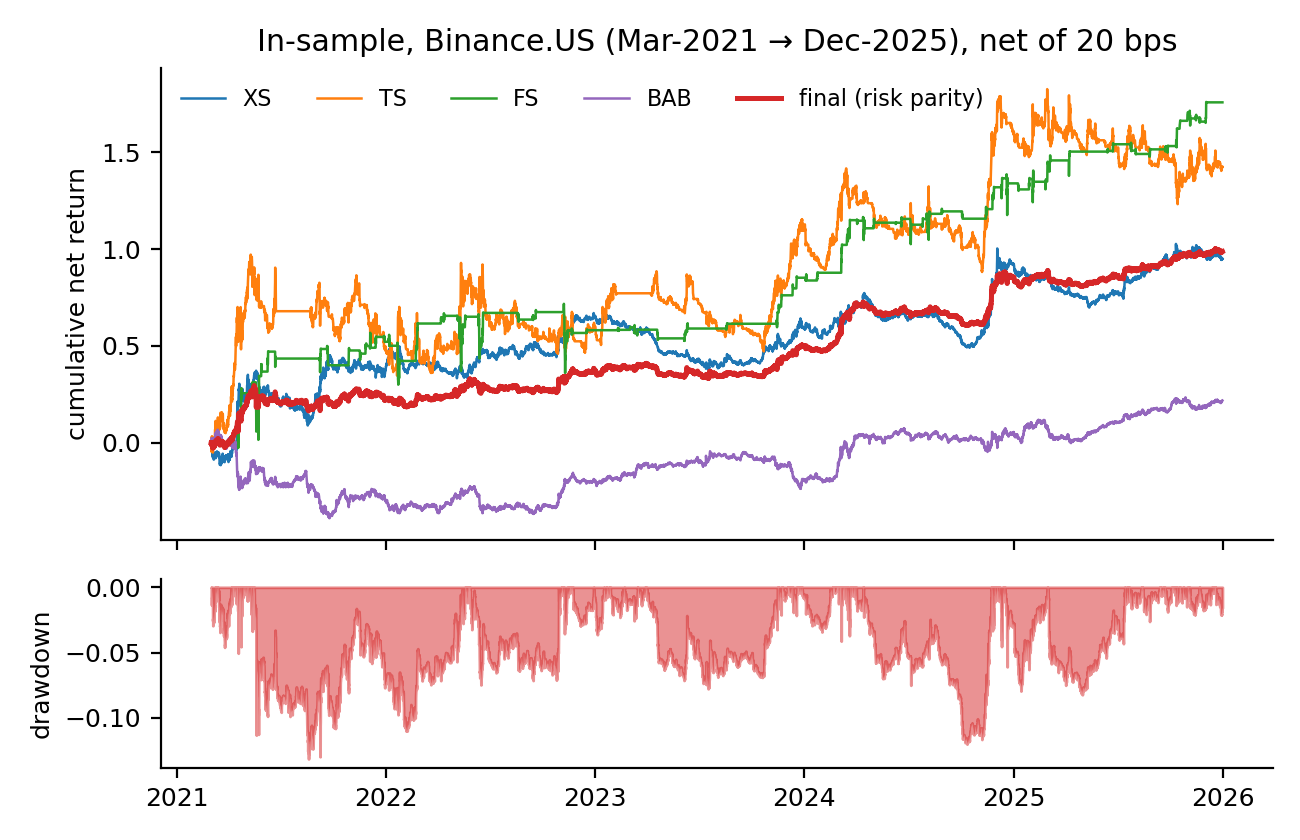
\includegraphics[width=0.85\linewidth]{figures/f3_insample.png}
		\caption{Cumulative net return (summed, 20~bps) of the four strategies and the risk-parity combination on Binance.US, and drawdown of the combination.}
		\label{fig:insample}
	\end{figure}
	
	\begin{table}[!htbp]
		\caption{Final strategy (4 strategies, risk parity), Binance.US, March 2021 -- December 2025.}
		\label{tab:final}
		\begin{ruledtabular}
			\begin{tabular}{lc}
				Net Sharpe (20 bps)  & 1.43 \\
				Annual return        & 20.4\% \\
				Annual volatility    & 14.3\% \\
				Max drawdown         & $-13.1\%$ \\
			\end{tabular}
		\end{ruledtabular}
	\end{table}

	\begin{table}[!htbp]
		\caption{Regression of the 4-hour net returns of the final strategy on the equal-weight market and on BTC, Binance.US, March 2021 -- December 2025.}
		\label{tab:alpha}
		\begin{ruledtabular}
			\begin{tabular}{lcc}
				Factor              & Equal-weight market & BTC \\
				\hline
				Beta                & 0.061  & 0.075 \\
				Annual alpha        & 17.7\% & 18.3\% \\
				$t$-stat (alpha)    & 2.89   & 2.95 \\
			\end{tabular}
		\end{ruledtabular}
	\end{table}
	
	\begin{table}[!htbp]
		\caption{Net Sharpe ratio by year, Binance.US.}
		\label{tab:yearly}
		\begin{ruledtabular}
			\begin{tabular}{lccccc}
				Year & XS & TS & FS & BAB & Final \\
				\hline
				2021 & 1.25    & 0.82    & 1.34 & $-1.41$ & 1.26 \\
				2022 & 1.25    & 0.17    & 0.14 & 0.68    & 1.20 \\
				2023 & $-0.34$ & 1.27    & 2.09 & 0.07    & 1.30 \\
				2024 & 1.33    & 0.96    & 1.32 & 1.37    & 2.24 \\
				2025 & 0.15    & $-0.32$ & 1.47 & 1.19    & 1.29 \\
			\end{tabular}
		\end{ruledtabular}
	\end{table}
	
	% =====================================================================
	\section{Out-of-sample test on Binance global data}
	\label{app:oos}
	
	Binance.US volume collapsed in 2026 (e.g.\ VET $\approx \$33$ and ATOM $\approx \$17$ per hour), so all four strategies were rebuilt from Binance global prices for the same 13 coins with exactly the same rules and parameters (data from the public mirror \texttt{data-api.binance.vision}). The year 2025 was partly visible during development; 2026 was never seen.
	
	\begin{figure}[!htbp]
		\centering
		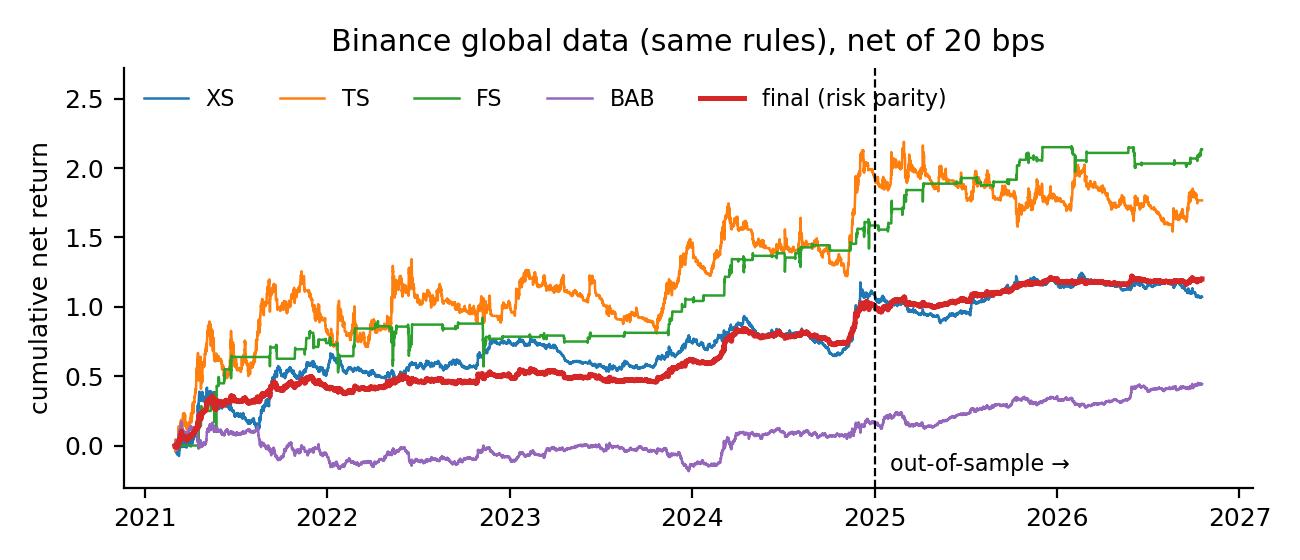
\includegraphics[width=0.85\linewidth]{figures/f4_oos.png}
		\caption{Cumulative net return (20~bps) on Binance global data. The dashed line marks the start of the out-of-sample period.}
		\label{fig:oos}
	\end{figure}
	
	\begin{table}[!htbp]
		\caption{Net Sharpe ratio on Binance global data.}
		\label{tab:oos}
		\begin{ruledtabular}
			\begin{tabular}{lcccc}
				Strategy & In-sample 2021--24 & 2025 & 2026 (Jan--Oct) & Out-of-sample 2025--26 \\
				\hline
				\textbf{Final (4 strategies)} & \textbf{1.73} & \textbf{1.96} & $\mathbf{-0.05}$ & \textbf{1.17} \\
				3 strategies, risk parity     & 1.77 & 1.35    & $-0.84$ & 0.56 \\
				XS                            & 1.15 & 0.57    & $-1.08$ & $-0.07$ \\
				TS                            & 0.82 & $-0.27$ & $-0.07$ & $-0.20$ \\
				FS                            & 1.11 & 2.20    & $-0.10$ & 1.34 \\
				BAB                           & 0.26 & 1.43    & 1.03    & 1.27 \\
			\end{tabular}
		\end{ruledtabular}
	\end{table}
	
	On global data the strategy holds in sample (1.73), so it is not an artifact of Binance.US prices. Out of sample the final portfolio earns a Sharpe of 1.17 with 9\% volatility and a $-8\%$ maximum drawdown. In 2026 it was flat ($-0.05$): XS momentum lost ($-1.08$), TS momentum and fire sale were about flat, and BAB (1.03) was the only winner. Momentum failed in 2026 because (i) coins moved together, with the lowest cross-sectional dispersion of 30-day returns of any year (0.09); (ii) the rank correlation between past and next 30-day returns was $-0.10$, the lowest of any year; and (iii) a sharp rebound inside a bear market ($+21\%$ and $+24\%$ in August--September after $-26\%$ in June) hit the short side, the momentum crash described by Daniel and Moskowitz~\cite{daniel2016}. Over 9.5 months the standard error of a Sharpe ratio is about 1.1, so 2026 alone is not statistically different from the in-sample result.
	
	% =====================================================================
	\section{Limitations}
	\label{app:limits}
	
	The universe is small (13 coins) and the history short (6 years); many specifications were tried on the same data, so in-sample Sharpe ratios are optimistic. Costs are a single 20~bps estimate, capacity on Binance.US is very small, shorting requires perpetual futures or margin whose funding costs are not modeled, the coin filter uses full-sample volume, and weight drift between rebalances is ignored. Netting the trades of the four strategies into one book would save about 10\% of costs (estimated Sharpe 1.41 instead of 1.35 for the three-strategy combination).
	
	\begin{thebibliography}{2}
		\bibitem{frazzini2014} A.~Frazzini and L.~H.~Pedersen, Betting against beta, \textit{J. Financ. Econ.} \textbf{111}, 1 (2014).
		\bibitem{daniel2016} K.~Daniel and T.~J.~Moskowitz, Momentum crashes, \textit{J. Financ. Econ.} \textbf{122}, 221 (2016).
	\end{thebibliography}
	
\end{document}
